\documentclass[12pt]{article}

\usepackage[hmargin=1in,vmargin=1in]{geometry}
\usepackage{parskip}
\usepackage{hyperref}
\usepackage{graphicx}
\usepackage{color}
\usepackage{verbatim}
\hypersetup{pdfstartview=FitV,hidelinks}



\begin{document}

{
  \Large
  \centering
  {\bf Lab 11 -- Estimating survival, recruitment, and growth rate
    with capture-mark-recapture data} \\
  Due before your next lab \par
}

\vspace{10pt}

% Analysis of the (fake) Mongolian gazelle ({\it Procapra gutturosa})
% data using program DISTANCE.

The purpose of this lab is to learn how to use program MARK to
estimate survival, recruitment, and growth rate using mark-recapture
data. Put your answers in a Word file named something like
``Chandler-lab11.docx'', and upload it to ELC.

\vspace{-12pt}


\section*{\large Exercise I: Estimating Canada Warbler survival with
  the CJS model}

\vspace{-10pt}

{\bf Background}

The Canada Warbler ({\it Cardellina canadensis}) is a long-distance
migratory bird that primarily breeds in the boreal forests of
Canada. However, a small portion of the range extends down through the
Appalachian Mountains to northern Georgia.

Canada Warblers are too small to use telemetry to estimate annual
survival, so we use mark-recapture methods instead. Each year, we
visit multiple sites and run mist-nets for 4 consecutive days at each
site. All newly captured individuals are marked with a uniquely
numbered metal band, and a unique combination of color bands.

The data come from five years (2014--2018) of surveys. Even though
``the robust design'' was used, the data were collapsed so that only
one value (0 or 1) is shown for each year for each individual. Program
MARK will ignore all leading zeros in the encounter histories.

{\bf Instructions}

\begin{enumerate}
  \item Create a New Project, name it \verb+"Exercise I"+, and select
    the \verb+"cawa-cjs.inp"+ data file.
  \item Choose the \verb+"Live Recaptures (CJS)"+ Data Type
  \item The number of \verb+"Encounter occasions"+ should be set to 5
  \item Hit \verb+"OK"+ and then \verb+"OK"+ again when the dialog box
    appears
  \item Use the \verb+"Run > Pre-defined Model(s) > Select Models"+
    option to run all four pre-defined models, which differ only in
    whether or not $p$  and $\phi$ vary over time. Hit \verb+"OK"+ and
    then \verb+"OK to Run"+.
\end{enumerate}

{\bf Assignment}

\begin{enumerate}
  \item What is the best model according to AICc?
  \item Create a table to report the estimates, standard errors, and
    95\% confidence intervals for $p$ and $\phi$ from the best model.
  \item Interpret the estimates of $p$ and $\phi$ using one sentence
    for each parameter.
  \item The estimate of $p$ is fairly low and imprecise. Describe two
    ways in which we could modify our design (and analysis) to improve
    our estimate of $p$.  
\end{enumerate}

  
\clearpage

\section*{\large  Exercise II: The Jolly-Seber model for estimating
  survival, recruitment, and growth rate}

\textcolor{red}{THE CH DATA HAVE CHANGED AND THERE ARE MORE THAN 5 SIX
  YEARS NOW. NEED TO FIX THIS}

{\bf Background}

Stinkpots ({\it Sternotherus odoratus}) were captured, marked,
released, and occasionally recaptured at Dean's Pond at
Whitehall Forest using baited hoop traps. Sampling began in 2007.


{\bf Instructions}

\begin{enumerate}
  \item Create a New Project, name it \verb+"Exercise II"+, and select
    the \verb+"CH-SO-Dean-AllYears.inp"+ data file.
  \item Choose the \verb+"Jolly-Seber"+ Data Type
  \item Set \verb+"Encounter Occasions"+ to 6 (for 6 years of data)
  \item Sampling occurred on years 2007, 2010, 2011, 2012, 2014, and
    2015, so the time intervals between sampling occasions differs. To
    account for this, select \verb+"Set Time Intervals"+ and specify the
    time gaps as 3, 1, 1, 2, 1. Hit \verb+"OK"+, then hit it again on
    the next screen.
  \item Close the next screen and then click
    \verb+"PIM > Change Data Type"+ and select the \\
    \verb+"Link-Barker Jolly-Seber"+ option. This lets us estimate
    survival ($\phi$), recruitment ($f$), and capture probability
    ($p$) rather than survival, growth rate and capture probability,
    which is the default option. 
  \item Use the \verb+"Run > Pre-defined Model(s) > Select Models"+
    option to fit at all 8 possible models, which differ in whether or
    not each parameter is constant or varies among years.
%  \item Right-click on the model with the lowest AICc
%  score and selected \verb+"Derived parameters"+ to view yearly
%  estimates of lambda ($\lambda_t$).
\end{enumerate}





% \begin{figure}[h!]
%   \centering
%   \fbox{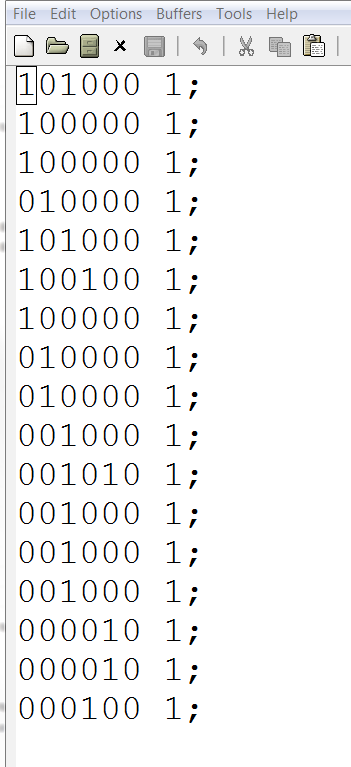
\includegraphics[height=7.5cm]{figs/stinkpot07-data}}
%   \caption{\small Stinkpot capture histories in a text file ready to
%     be imported to MARK.}
%   \label{fig:stink07-data}
% \end{figure}

{\bf Assignment}

\begin{enumerate}
  \item What is the best model in terms of AICc?
  \item Interpret the parameter estimates (\verb+"Real Estimates"+)
    from the model with the lowest AICc. (For parameters that are
    year-specific, you do not need to interpret each yearly-estimate.)
  \item What are the estimates of lambda ($\lambda_t$) for each time
    interval? These can be found by right-clicking on a model and
    choosing \verb+"Derived parameters"+.
%  \item What is the relationship between the estimates of survival,
%    recruitment and lambda?
  \item Bring the estimates of lambda into Excel and create a plot of
    lambda over time. Include this in your Word file.
  \item What conclusions can you draw from
    this analysis? Do you think the population is growing, shrinking,
    remaining constant, or is it difficult to tell?
%  \item How could you get more precise parameter estimates?
\end{enumerate}

% \begin{table}[h!]
%   \centering
%   \caption{A description of the four models to be fitted to the
%     stinkpot data.}
%   \footnotesize
%   \begin{tabular}[h!]{ll}
%     \hline
%     Model name & Model description \\
%     \hline
%     $M_0$ & The most basic model in which $p$ and $c$ are constant \\
%     $M_t$ & A model in which $p$ differs among sampling occasions and
%             $p_t=c_t$. \\
%     $M_b$ & A behavioral response model in which $p$ and $c$
%             differ. Can describe trap happiness or trap shiness. \\
%     $M_{tb}$ & A combination of models $M_t$ and $M_b$. \\
%     \hline
%   \end{tabular}
%   \label{tab:Otis}
% \end{table}


% \clearpage


% {\bf Parameter definitions}
% \begin{itemize}
%   \item $p$ -- capture probability. The probability of capturing an
%     individual on a single occasion
%   \item $p_t$ -- capture probability on occasion $t$
%   \item $\phi$ -- apparent survival probability. The probability of
%     surviving and not permanently emigrating from the study area
%   \item $N$ -- abundance. The number of individuals in the
%     population. $N=n+f_0$.
% \end{itemize}






\end{document}




